\section{Más funcionalidades útiles}
\frame
{
\frametitle{Más funcionalidades útiles}
\begin{itemize}
 \item \textbf{pull}\\ \indent
Utilizándolo sin ningún parámetro adicional -\textbf{git pull origin master}- funciona igual que un \textit{update} en Subversion. Es decir, se trae los cambios y hace \textit{merge}. Si le pasamos el parámetro \textit{-{}-rebase}, funciona como un \textit{rebase}.
\end{itemize}

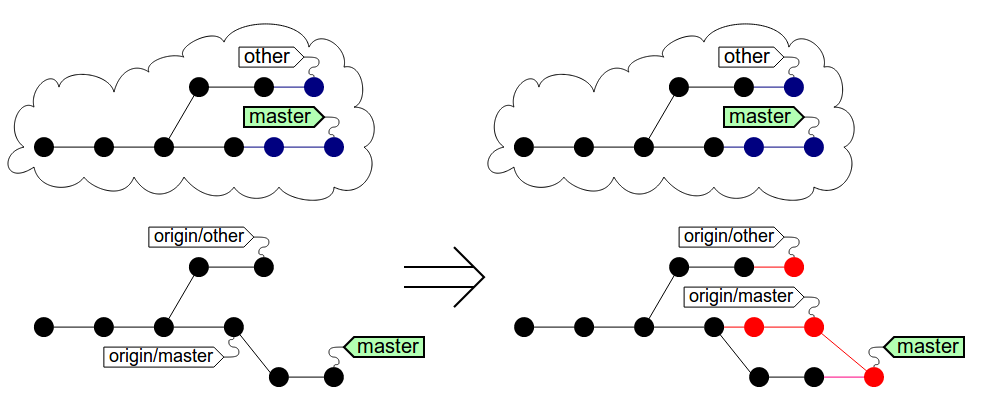
\includegraphics[height=5cm]{imgs/pull.png} 
}

\frame
{
\frametitle{Más funcionalidades útiles}
\begin{itemize}
 \item \textbf{gitignore}\\ \indent
Este fichero se suele colocar en la raíz del proyecto y el contenido suele ser un listado de elementos que no queremos que sean reconocidos como ficheros del repositorio. 
 \item \textbf{update-index -{}-assume-unchanged}\\ \indent
Este comando se utiliza para ficheros que accidentalmente se han \textit{comiteado} (y probablemente \textit{pusheado}) y no queremos tener en cuenta los cambios producidos en estos ficheros, ya que lo veremos como modificados en la etapa II (listo para \textit{comitear}).
\end{itemize}
}

\frame
{
\frametitle{Más funcionalidades útiles}
\begin{itemize}
 \item \textbf{revert}\\ \indent
  Este comando deshace un único commit aplicando el parche con la diferencia como un nuevo commit. Ejemplo: git \textbf{revert} HEAD
 \begin{tabular}{p{4cm}|p{4cm}}\\
    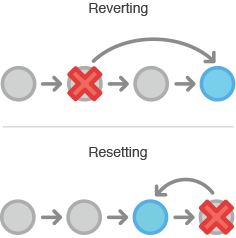
\includegraphics[height=4cm]{imgs/revert-vs-reset.png}&
    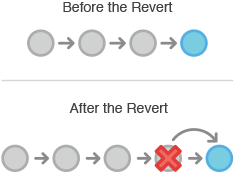
\includegraphics[height=3.5cm]{imgs/revert-sample.png}\\
 \end{tabular}
\end{itemize}

 Este comando no destruye la historia ni diverge las ramas \textit{master}. Ejemplo pack commits: git \textbf{revert} master\textasciitilde2..master
}

\frame
{
\frametitle{Más funcionalidades útiles}
\begin{itemize}
 \item \textbf{soft reset}\\ \indent
 El comando git reset -{}-soft <hash> mueve el puntero de la cabeza al hash del commit que le indiquemos.\\
 \begin{center}
    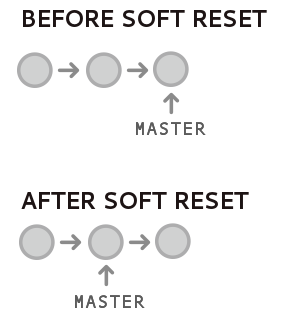
\includegraphics[height=4cm]{imgs/soft-reset.png}
 \end{center}
\end{itemize}
}

\frame
{
\frametitle{Más funcionalidades útiles}
\begin{itemize}
 \item \textbf{hard reset}\\ \indent
 El comando git reset -{}-hard <hash> mueve el puntero de la cabeza al hash del commit que le indiquemos y \textbf{destruye} toda la historia hasta dicho hash.\\
 \begin{center}
    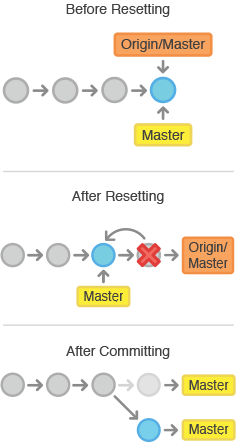
\includegraphics[height=6cm]{imgs/reset-hard.png}
 \end{center}
\end{itemize}
}

\section{Algo más avanzado}
\frame
{
\frametitle{Algo más avanzado}
\begin{itemize}
 \item squash
 \item format-patch
 \item cherry-pick
 \item stash
 \item reflog 
 \item submodules
 \item lolcommits 
\end{itemize}
}
